%\section{Ergebnisse}
%
\section{Ergebnisse der Kalibrierung}
\label{sec:calibrationResults}
%
Es werden die Ergebnisse der Kalibrierung vorgestellt. Für eine der vermessenen Antennenkonfigurationen sind in der folgenden Tabelle die Koordinaten der Antennen gezeigt. Die Visualisierung der Konfiguration zeigt die Abbildung~\ref{fig:3dplot_coordinates}.
%
\begin{table} [ht]
	\begin{center}
		\begin{tabular}{cccccccc}
		      \textbf{Antenne} & \textbf{$x$} & \textbf{$y$} & \textbf{$z$} & \textbf{$d_{meas}$} & \textbf{$d_{result}$}& \textbf{$\varepsilon_{abs}$} & \textbf{$\varepsilon_{rel}$} \\
		      1 & 0.48		& -1.01	& 0.60 & 1,259 & 1,274& 0,015 & 1,14\% \\
		      2 & -0.77 	& -1.04 	& 1.34 & 1,894 & 1,872 & -0,022 & 1,19\% \\
		      3 & 1.52  	& -1.05 	& 1.37 & 2,334 & 2,307 & -0,027 & 1,15\% \\
		      4 & -0.92 	& -0.19 	& 1.32 & 1,661 & 1,628 & -0,033 & 2,01\% \\
		      5 & 1.92 		&  0.03 	& 1.39 & 2,399 & 2,375 & -0,024 & 1,01\% \\
		      6 & -0.55 	&  1.09 	& 1.43 & 1,851 & 1,887 & 0,036 & 1,93\% \\
		      7 & 1.06 		&  1.07 	& 1.35 & 2,055 & 2,031 & -0,024 & 1,19\% \\
		      8 & 0.45 		&  1.35 	& 0.67 & 1,574 & 1,578 & 0,004 & 0,26\% \\					
%
		\end{tabular}
		\caption[Finale Antennen Koordinaten]{Tabelle der finalen Antennenkoordinaten [m], berechnet mit dem in dieser Arbeit entwickelten Modell und dem SVD-Verfahren. Die Ergebnisse wurden auf zwei Nachkommastellen gerundet und sind identisch für beide Methoden. Die Spalte $d_{result}$ enthält die von der Berechnung gefundenen Distanz vom Referenzpunkt zur Antenne. Die Spalte $d_{meas}$ zeigt die gemessenen Werte. Die $\epsilon$-Spalten zeigen die Abweichung.}
		\label{tab:FinalCoords}
	\end{center}
\end{table}
%
Eine Berechnung mit dem evolutionären Verfahren dauerte ca. $170$~ms mit dem SVD-verfahren wurde eine Lösung in $\le 1$~ms gefunden. Für die in der Praxis eingesetzte Software wird es eine Implementation der Kalibrierung mit dem SVD-Verfahren geben. Das mit dieser Variante berechnete Ergebnis wird bei Bedarf mit einer Lösung des evolutionären Verfahrens verglichen. Das ermöglicht eine Build-In Verifikation der Kalibrierung.\\

\subsection{Visualisierung der Ergebnisse}
Für die in den folgenden Abbildungen präsentierten Ergebnisse wurden insgesamt $100$ Durchläufe des Algorithmus erstellt. Die Ergebnisse wurden mit einem vom Algorithmus selbst erstellten $\mu$ und $\lambda$ gefunden. In Abbildung~\ref{fig:Final_Calibration_Ant0_ES-boxes} wird eine statistische Auswertung der Ergebnisse gezeigt. In jedem Plot werden die Endwerte der Lösungen in einem sog. Boxplot gezeigt. Dabei wird die Verteilung mit Hilfe von Boxen dargestellt. Die Fähnchen der Boxen stellen die maximal- bzw. minimal-Werte dar. Die Größe der Boxen enthält das obere und untere Quartil der Daten, der horizontale Strich in der Box zeigt den Mittelwert der Daten. Ausreißer\footnote{Hier Werte die mindestens den $2$-Fachen Wert des oberen- bzw. unteren-Quartils aufweisen} in den Daten werden durch Punkte abseits der Box dargestellt.\\
%

Die Abbildung~\ref{fig:Final_Calibration_Ant0_ES-boxes} zeigt den Verlauf der drei Objektvariablen ($x,y,z$-Koordinaten) sowie die Entwicklung der Fitness und des mittleren Sigmas. Als Darstellungsart wird der Linienplot verwendet und die Verläufe einzelner Lösungen überlagern sich in diesem Plot. Das Abbruchkriterium war eine Fitness von $\leq 10^{-25}$.% Ist Fitness nicht etwas gutes und sollte maximiert werden?
Für Darstellungszwecke wurde die $x$-Achse nach $500$ Werten beschränkt, daher erreicht der Fitness-Plot diesen Wert in der Abbildung nicht. Der Verlauf ist typisch für den verwendeten Algorithmus. Deutlich zu erkennen ist eine Verbesserung des Ergebnisses mit steigender Zahl der Generationen. Der Verlauf der Variablen ist immer für den erfolgreichsten Nachkommen einer Generation dargestellt.\\
%

Abbildung~\ref{fig:Final_Calibration_Ant0_ES-Scatter} ist ein Scatter-Plot. Die Objektvariablen werden hier gegeneinander aufgetragen. Auf der Diagonalen befinden sich stets die Variable gegen sich selbst aufgetragen, daher zeigt sich dort immer eine Linie, bei streuenden Ergebnissen, bzw. ein einzelner Punkt, sollten die Ergebnisse nicht streuen. Der Plot ist praktisch um die Implementation des Algorithmus zu verifizieren. Er lässt Rückschlüsse auf Abhängigkeiten und Einflüsse der Objektvariablen zu. So können die Ergebnisse mit den Erwartungen an die Verläufe verglichen werden.\\
%
%---------------------------------------------------------------
%
\begin{figure}[!ht]
  \begin{center}
   \caption[Box-Plot der Endergebnisse der Kalibierung]{Boxplot des Kalibierergebnis aus $100$ Durchläufen. Im oberen Plot sind die x,y,z-Koordinaten gezeigt, diese landen in allen Durchläufen auf dem selben Ergebnis. Was nicht verwundert, das Problem ist eines der Art \glqq{}drei Gleichungen und drei Unbekannte\grqq. Die Streuung der Lösung zeigt sich in der Breite der Linien. Die unteren vier Plots zeigen die Anzahl der Evaluationen der Fitness-Funktion, den finalen Funktionswert, das Sigma für die Variablen und die Entfernung zum Referenzpunkt (v.l.n.r.). Das Ergebnis sind die Koordinaten für Antenne 1}
    \label{fig:Final_Calibration_Ant0_ES-boxes}
    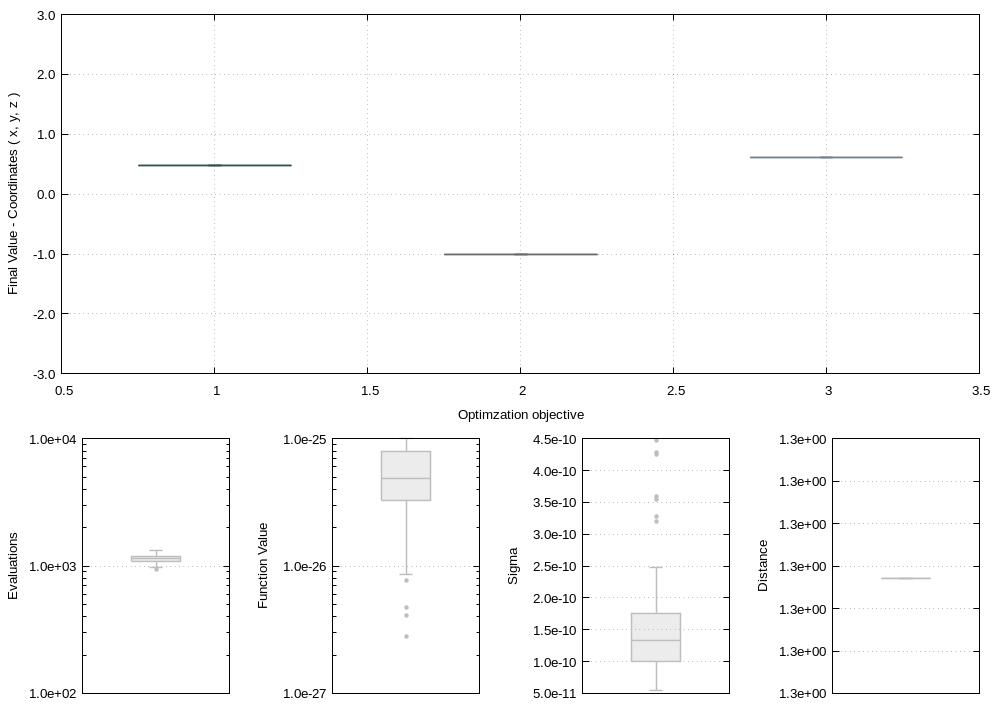
\includegraphics[width=0.9\textwidth]{img/calibration/calibration_ant0-boxes.png}
  \end{center}
 
%
\end{figure}
%
%---------------------------------------------------------------
%
\begin{figure}[!ht]
  \begin{center}
    \caption[Linien-Plot der Endergebnisse der Kalibierung]{Zu erkennen ist, dass nach ca. 300 Evaluationen der Zielfunktion keine großen Änderungen der Variablen zu erkennen sind. Bis zum erreichen des Abbruchkriteriums (Function Value $\leq10^{-25}$) werden noch ca 400 Evaluationen benötigt, vgl. korrespondierender Boxplot.}
    \label{fig:Final_Calibration_Ant0_ES-Lines}  
    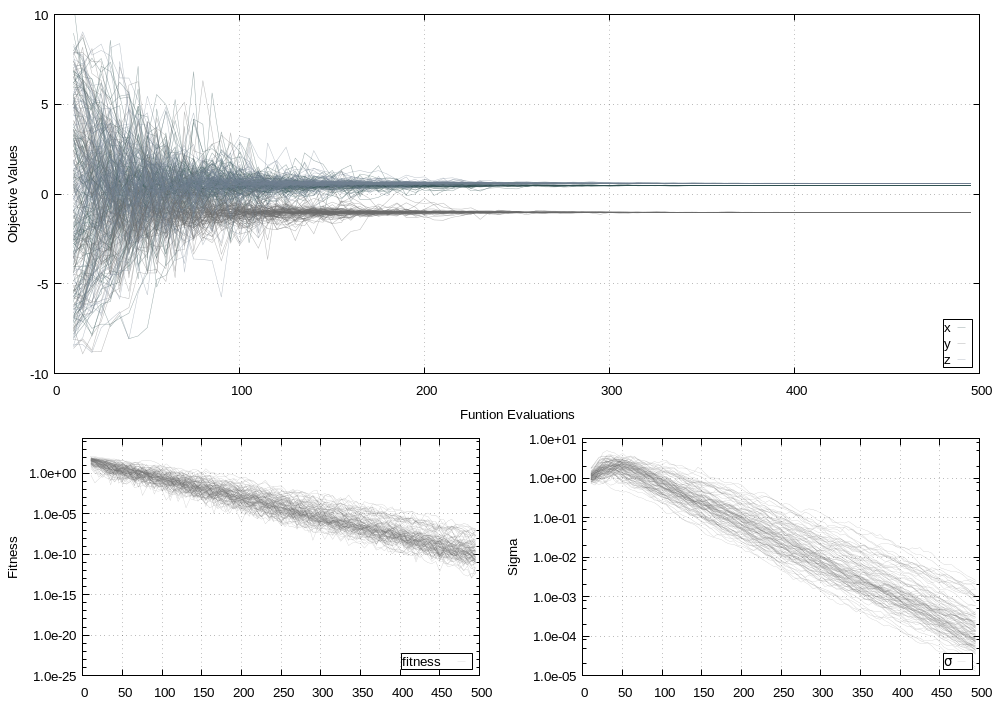
\includegraphics[width=0.9\textwidth]{img/calibration/calibration_ant0-lines.png}
  \end{center}
%  
\end{figure}
%---------------------------------------------------------------
%
\begin{figure}[!ht]
  \begin{center}
  
    \caption[Kalibierung Scatter-Plot]{Scatter-Plot der Ergebnisse der evolutionären Kalibrierung. Die Endergebnisse streuen in keiner Dimension, das wird aus dieser Darstellung deutlich.}
    \label{fig:Final_Calibration_Ant0_ES-Scatter}  
    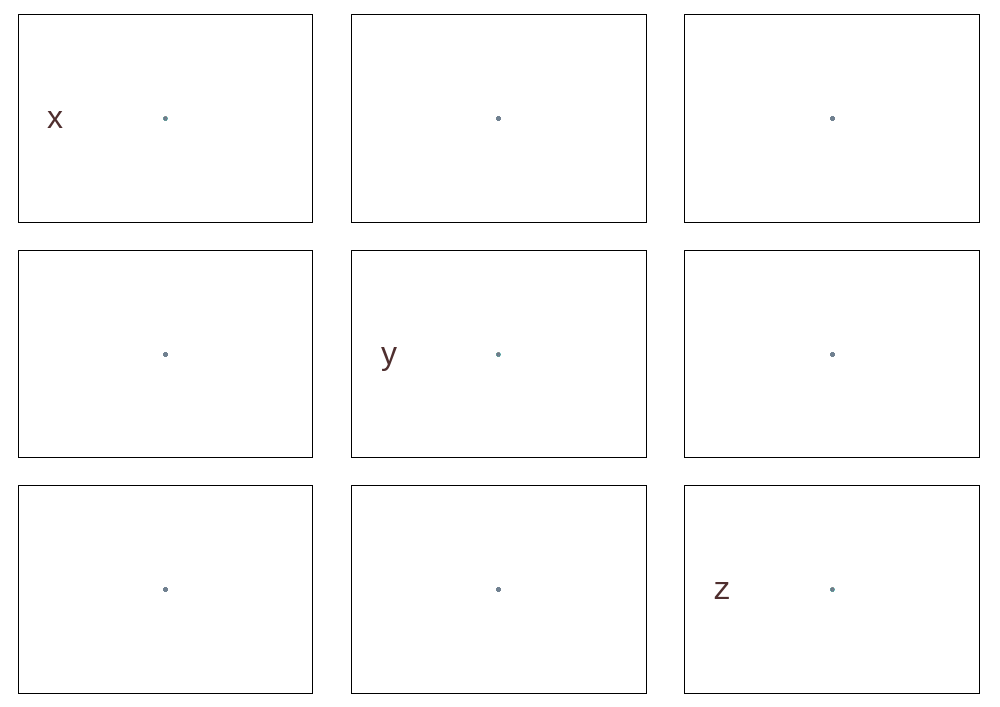
\includegraphics[width=0.9\textwidth]{img/calibration/calibration_ant0-scatter.png}
  \end{center}
%  
\end{figure}
%---------------------------------------------------------------
%
\begin{figure}[!ht]
     \centering
     \begin{subfigure}[t]{0.45\textwidth}
             \centering
             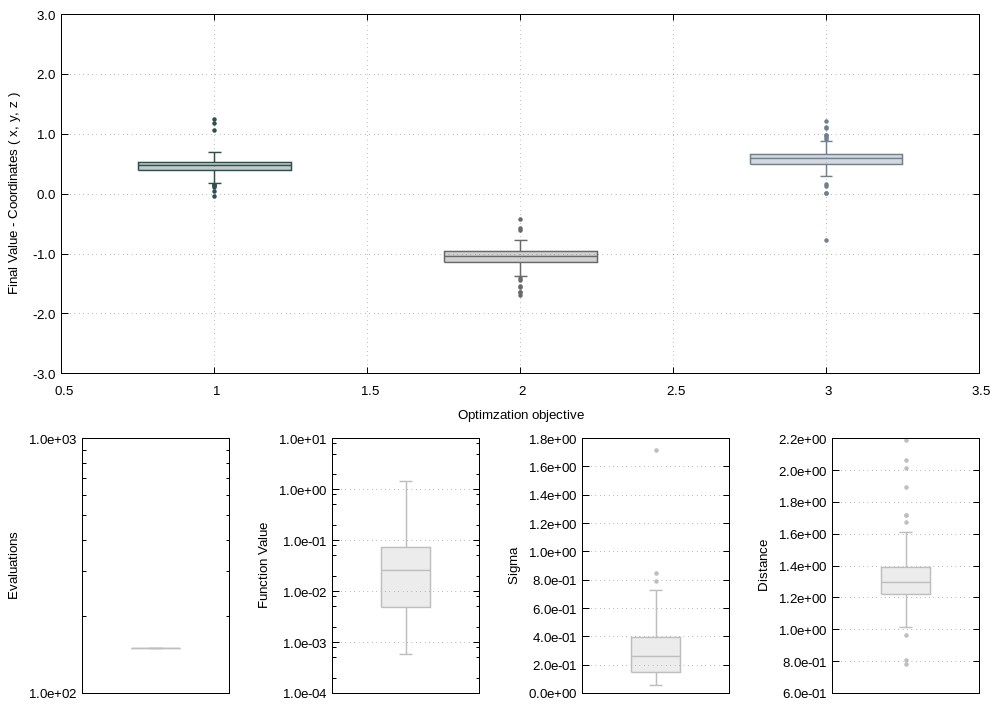
\includegraphics[width=\textwidth]{img/calibration/aborted_calibration_ant0-boxes.png}
             \caption{Statistisch verteilte Endwerte für die Koordinaten der Kalibrierung.}
             \label{fig:abortedFinal_Calibration_Ant0_ES-boxes}
     \end{subfigure}
%
\qquad         
%
     \begin{subfigure}[t]{0.45\textwidth}
             \centering
             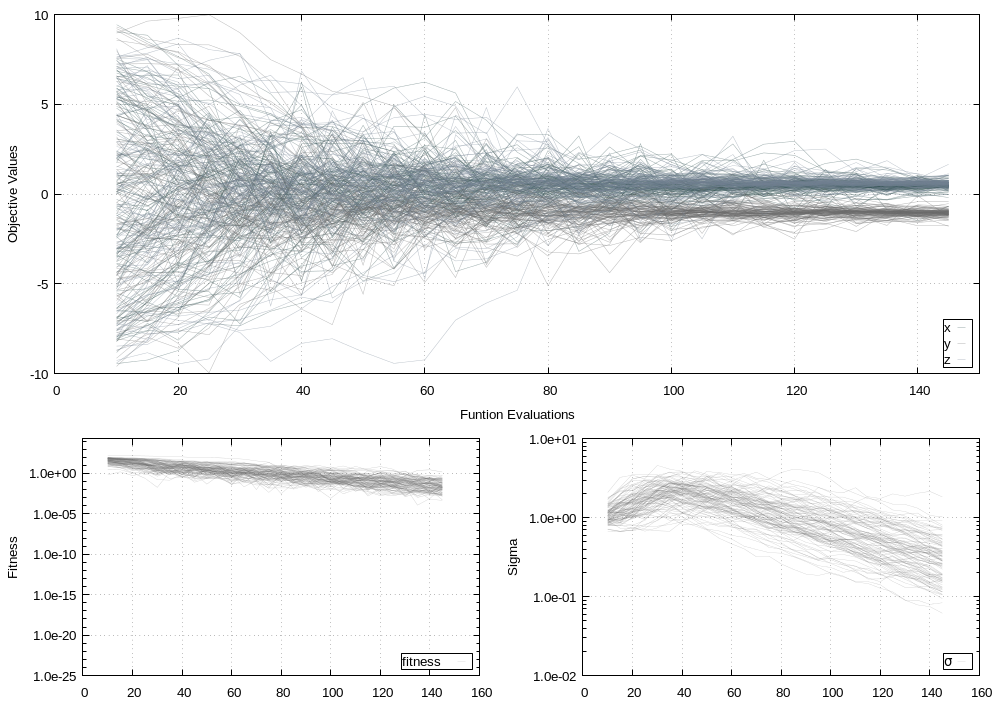
\includegraphics[width=\textwidth]{img/calibration/aborted_calibration_ant0-lines.png}
             \caption{Linienplot der bei $140$ Evaluationen abgebrochenen Verläufe. Gut zu sehen ist der Verlauf der Objektvariablen, die sich von Generation zu Generation dem realen Wert nähern.}
             \label{fig:abortedFinal_Calibration_Ant0_ES-Lines}
     \end{subfigure}
%
\\
%
     \begin{subfigure}[t]{0.4\textwidth}
             \centering
             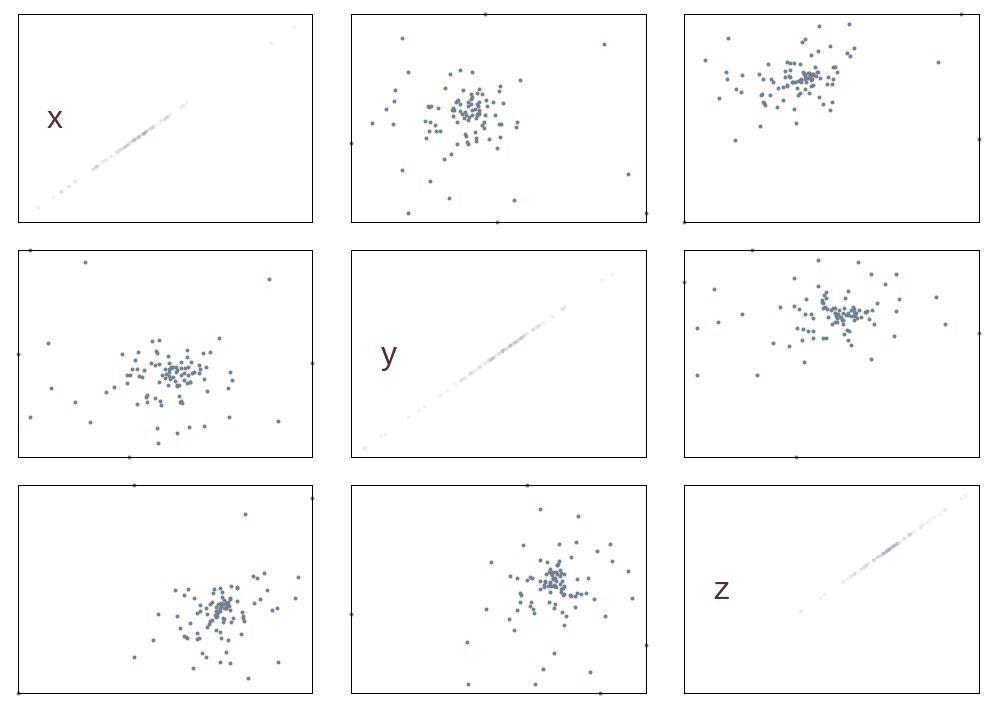
\includegraphics[width=\textwidth]{img/calibration/aborted_calibration_ant0-scatter.png}
             \caption{Statistische Streuung um einen Mittelwert. So in etwa kann man die Lösungen der Komplexen Probleme erwarten.}
             \label{fig:abortedFinal_Calibration_Ant0_ES-Scatter}
     \end{subfigure}
%
     \caption[Statistisch verteilte Ergebnisse der Kalibrierung mittels ES]{Analog zu den Abbildungen~\ref        {fig:abortedFinal_Calibration_Ant0_ES-Lines}, \ref{fig:abortedFinal_Calibration_Ant0_ES-boxes} und \ref{fig:abortedFinal_Calibration_Ant0_ES-Scatter} zeigen die Plots die gleichen Darstellungen. Hier gezeigt wird, wie sich eine statistische Verteilung in den Plots manifestieren würde. Um das zu demonstrieren wurde das Abbruchkriterium auf lediglich $150$ Evaluationen der Zielfunktion eingestellt. Zu diesem Zeitpunkt können die Objektvariablen bereits einen passablen Wert erreicht haben oder noch abweichende Werte aufweisen (vgl. \ref{fig:Final_Calibration_Ant0_ES-Lines}).}
     \label{fig::abortedFinal_Calibration_Ant0_ES}
\end{figure}
%
\begin{figure}[ht!]
         \centering
         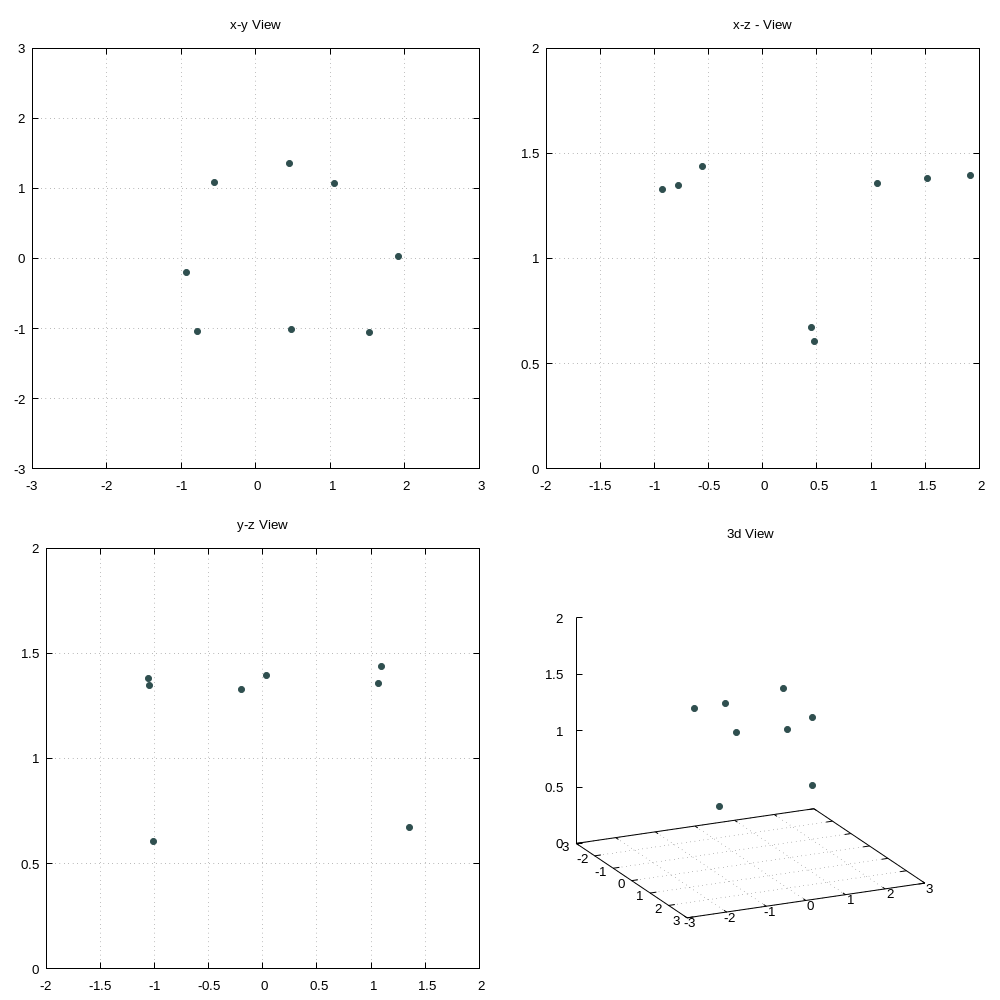
\includegraphics[width=0.7\textwidth]{img/calibration/calibration_results.png}
         \caption[Visualisierung des Kalibrierendergebnis]{Visualisierung des Kalibrierendergebnis. Abgebildet sind die gefundenen Antennenkoordinaten (Punkte) in drei Raumansichten. Die zusätzliche, dreidimensionale  Ansicht dient der Übersicht. Das Ergebnis und die reale Anordnung decken sich sehr gut. Siehe Tabelle~\ref{tab:FinalCoords}}
         \label{fig:3dplot_coordinates}
%
\end{figure}

Das Modell aus \ref{sec:model_developement} wurde in verschiedenen Experimenten untersucht. Dabei wurden die Parameter der Optimierung variiert und die Auswirkungen untersucht.

Es wird analysiert, wie gut die Lösbarkeit des unregistrierten Problems ist. Dazu werden zuerst für jede Referenzantenne immer eine mögliche Konfiguration gewählt und das Ergebnis aus $M$-Durchläufen untersucht. Im Anschluss %MENE: trinken wir Bier! %CG: DAS MACHEN WIR!

Zunächst werden die Ergebnisse der Experimente für idealen Messwerte vorgestellt, dannach wird dieselbe Darstellung für reale Messdaten vorgenommen. Die Darstellung der Ergebnisse ist eine kondensierte Form der Präsentation. Sie Zeigen 
%
%-----------------------------------------------------------------------------
%
\section{Ergebnisse des Trilaterationsmodells}
%
\label{sec:Results1}
%
Dieser Abschnitt enthält die Ergebnisse der evolutionären Optimierung für das entwickelte Modell der Trilateration. Es werden Experimente definiert und ihre Resultate als Falschfarbenbild (Heatmap) dargestellt. Es werden die Ergebnisse von künstlichen Eingabedaten und realen Messdaten verglichen. Im Anschluss wird der Verlauf der Optimierung auf Besonderheiten hin untersucht. Abschließend wir die Performance der evolutionären Lösung visualisiert.
%
\subsection{Experimente}
%
Die Tabellen~\ref{tab:experiments} und~\ref{tab:experiments2} geben an welche Parameter wie variiert wurden. Diese Experimente wurde für die Präsentation der Ergebnisse in dieser Arbeit entworfen. Alle wurden mit der gleichen Objektfunktion durchgeführt. Diese trägt den Namen '\textit{WholeTomatoMkII}'\footnote{Implementation des in dieser Arbeit entwickelten Trilaterationsmodells}. Der eingesetzte Algorithmus ist das CMA-ES. Andere evolutionäre Strategien werden nicht in separaten Experimenten untersucht und präsentiert. Die spätere Darstellung kondensieren die Parameter und Erkenntnisse die in dieser Arbeit gewonnen wurden. Ziel ist es insgesamt die Lösung zu quantifizieren. Wie im Rahmen der Komplexitätsuntersuchung beschrieben ist die Fragestellung die hier bearbeitet wird recht komplex. Es werden daher die Parameter der Evolutionsstrategie variiert. Dabei wird untersucht ob und wie sich die Güte der Lösung durch diese Parameter verbessern lässt. In den Abbildungen~\ref{fig:results1} und~\ref{fig:results2} sind die Ergebnisse der Experimente als Heatmap dargestellt.

%
\begin{table} [ht!]	
	\caption[Experimente - Ideale Messdaten]{Aufstellung der Experimente die in diesem Abschnitt vorgestellt werden. Die Gruppengröße wird bei jedem Experiment Variiert. Jedes Unterexperiment erhält seinen eigenen Namen. Daher steigt der Name der Experimente bei jedem Eintrag entsprechend der Anzahl der untersuchten Gruppen an. In dieser Untersuchung wurden auch Parameter des Evolutionären Algorithmus variiert. Es werde $\mu$ und $\lambda$ variiert. Der Einfluss der Populations- und Gruppengröße wird damit gleichzeitig untersucht. Es ergeben sich $100$ einzelne Experimente.}
	\label{tab:experiments}
	\begin{center}
		\begin{tabular}{ccccc}
			\textbf{Name} 	& \textbf{Trials $M$} 	& \textbf{Gruppengröße $L$} & \textbf{$\mathbf{\mu}+\mathbf{\lambda}$}\\
			E2000			& 50 				&    1-10		&  (30+100) \\
			E2010			& 50 				&    1-10		&  (40+150) \\
			E2020			& 50 				&    1-10		&  (50+200) \\
			E2030			& 50 				&    1-10		&  (60+250) \\
			E2040			& 50 				&    1-10		&  (70+300) \\			                        
			E2050			& 50 				&    1-10		&  (80+350) \\			                        
			E2060			& 50 				&    1-10		&  (90+400) \\			                        
			E2070			& 50 				&    1-10		&  (100+450) \\			                        
			E2080			& 50 				&    1-10		&  (110+500) \\			                        
			E2090			& 50 				&    1-10		&  (120+550) \\			                        
%			
		\end{tabular}
	\end{center}
\end{table}
%

\begin{table} [ht!]	
	\caption[Experimente - Reale Messdaten]{Für bestmögliche Vergleichbarkeit wurden diese Experimente mit den gleichen Parametern durchgeführt wie die für ideale Daten. In diesem Experiment werden die realen Messwerte des PRPS in der Positionsberechnung verwendet. }
		\label{tab:experiments2}
	\begin{center}
		\begin{tabular}{ccccc}
			\textbf{Name} 	& \textbf{Trials $M$} 	& \textbf{Gruppengröße $L$} & \textbf{$\mathbf{\mu}+\mathbf{\lambda}$}\\
			E3000			& 50 				&    1-10		&  (30+100) \\
			E3010			& 50 				&    1-10		&  (40+150) \\
			E3020			& 50 				&    1-10		&  (50+200) \\
			E3030			& 50 				&    1-10		&  (60+250) \\
			E3040			& 50 				&    1-10		&  (70+300) \\			                        
			E3050			& 50 				&    1-10		&  (80+350) \\			                        
			E3060			& 50 				&    1-10		&  (90+400) \\			                        
			E3070			& 50 				&    1-10		&  (100+450) \\			                        
			E3080			& 50 				&    1-10		&  (110+500) \\			                        
			E3090			& 50 				&    1-10		&  (120+550) \\			                        
%			
		\end{tabular}
	\end{center}
\end{table}
%
%-----------------------------------------------------------------------------
%
\subsection{Ergebnisse ideale Messwerte}
%
\begin{figure}[h!]
	\centering
	\caption[Ergebnis-Heatmap - Ideale Messwerte]{ Ergebnisse verschiedener Experimente mit idealen Messwerten. Die Abbildung zeigt farbkodiert den Betrag der Abweichung vom wahren Wert der Entfernung (Ausgemessen). Zu beachten gilt, dass die Farbskala eine unterschiedliche Skalierung hat und somit jede Antenne separat betrachtet werden muss. Die Parameter die in diesen Experimenten variiert wurden sind die Populationsgröße ($\mu$ und $\lambda$) und die Gruppengröße $L$. Mit der $x$-Achse steigt die Populationsgröße an. Die $y$-Achse trägt die steigende Gruppengrößen auf.}
	\label{fig:results1}
	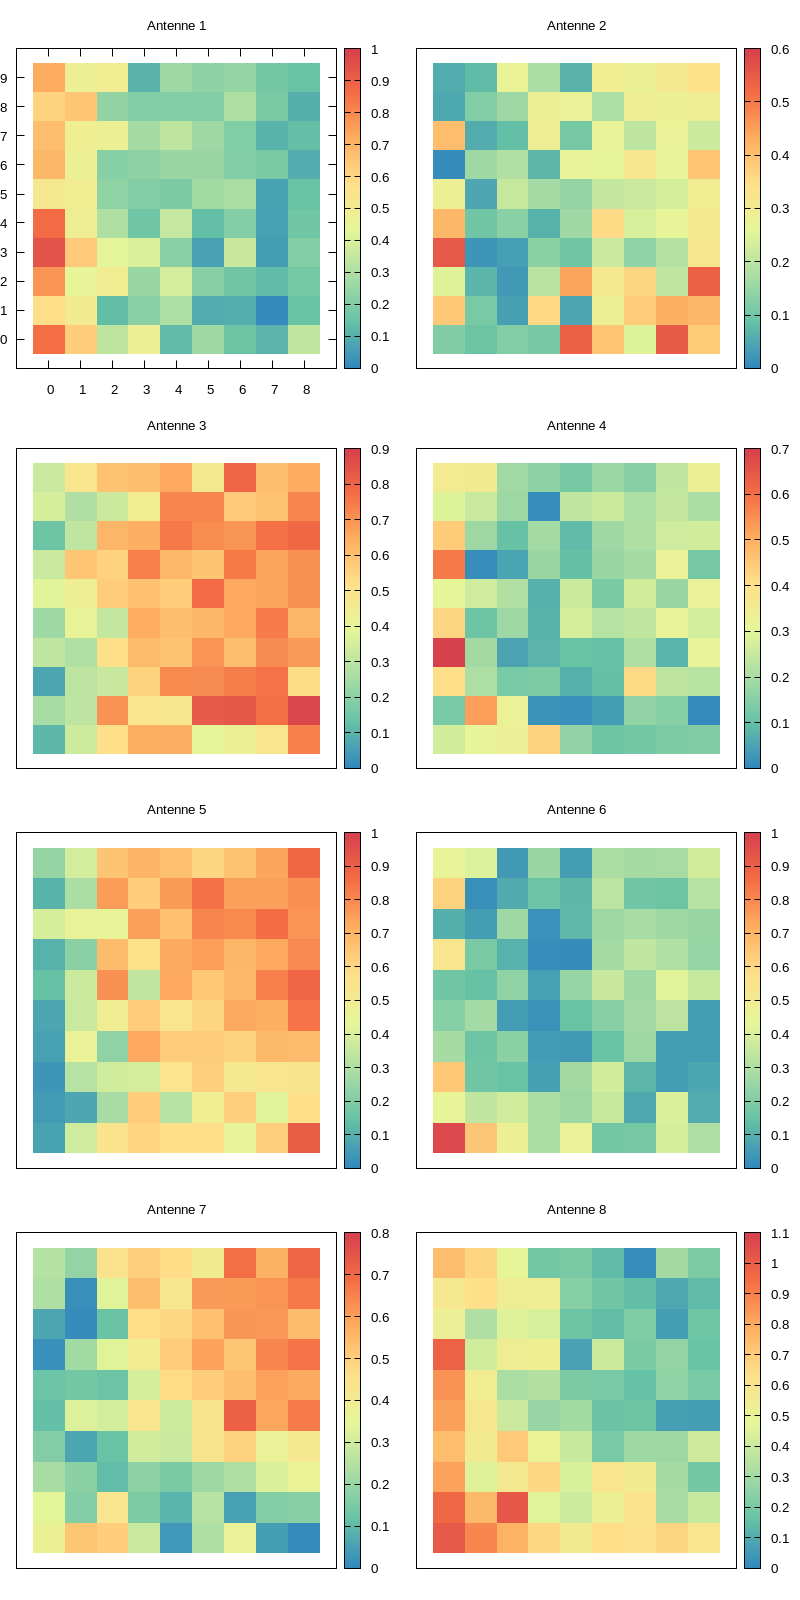
\includegraphics[width=0.65\textwidth]{img/result.png}
\end{figure}
% 
Um die idealen Messwerte zu generieren wurde ein eigenes Modul entwickelt. Es verwendet die in Kapitel~\ref{sec:PhaseCalculation} beschrieben Formeln. Es wurden eine Reihe von Punkten definiert, von denen die idealen Phasenwerte ermittelt wurden. Um im Rahmen dieser Arbeit in der Präsentation der Ergebnisse konsistent zu bleiben, wird als Punkt der Ursprung der Kalibrierung genutzt. Dieser muss von dem Algorithmus wiedergefunden werden. Seine Koordinaten wurden bereits in Kapitel~\ref{sec:calibration} besprochen. Die in den Abbildungen gezeigte Darstellung stellt die Abweichung von dem korrekten Wert dar.
%
$$
\varepsilon=~|~d_{true}-d_{found}~|
$$
%
Die Dimension von $\varepsilon$ ist dementsprechend [m]. Für die Visualisierung wurden auf den bestimmten $M$-Lösungen der Median-Wert (mittlere) genommen. 
%
\subsection{Ergebnisse ideale Messwerte}
%
Die idealen Messewerte zeigen insgesamt ein gutes Ergebnis (Abbildung~\ref{fig:results1}). Im Mittel werden die besten Ergebnisse, bei mittlerer Gruppengröße und großer Populationsgröße gefunden. Es zeigt sich, dass eine steigende Populationsgröße das Ergebnis in der Regel verbessert. Bei der Gruppengröße kann ab einer bestimmten Größe keine weitere Verbesserung festgestellt werden. Eine Besonderheit zeigt sich bei den Antennen $3$ und $5$. Diese zeigen ein umgekehrtes Verhalten, bei niedriger Gruppengröße und kleiner Populationsgröße zeigen sie die geringste Abweichungen. Woran das liegt konnte nicht weiter untersucht werden. Die meisten Lösungen zeigen eine Abweichung von unter einer Wellenlänge, die wir mit $\lambda\simeq35$~cm angeben konnten. Das erlaubt prinzipiell eine korrekte Berechnung der Wellenzahl.\\

In Abbildung~\ref{fig:results4} wurden die Ergebnisse anders eingefärbt, es werden Abweichungen über $35$~cm konsequent rot eingefärbt. Damit zeigt sich deutlicher, dass eine recht große Population und eine geeignete Gruppengröße gewählt werden muss um vernünftige Resultate zu erhalten.
%
%-----------------------------------------------------------------------------
%
\subsection{Ergebnisse reale Messwerte}
%
\begin{figure}[h!]
	\centering
	\caption[Ergebnis-Heatmap - Reale Messwerte]{ Ergebnisse mit realen Messwerten. Die Antennen $2$ und $6$ lieferten bei dieser Messung keine Messdaten. Daher fehlen diese Plots in der Grafik. Das Antennen keine Daten liefern ist der Regelfall den man in der Praxis begegnet. Das Ergebnis ist in etwa identisch mit dem der idealen Messwerte. Auch hier finden sich gute Ergebnisse bei mittlerer Gruppen- und großer Populationsgröße.}
	\label{fig:results2}
	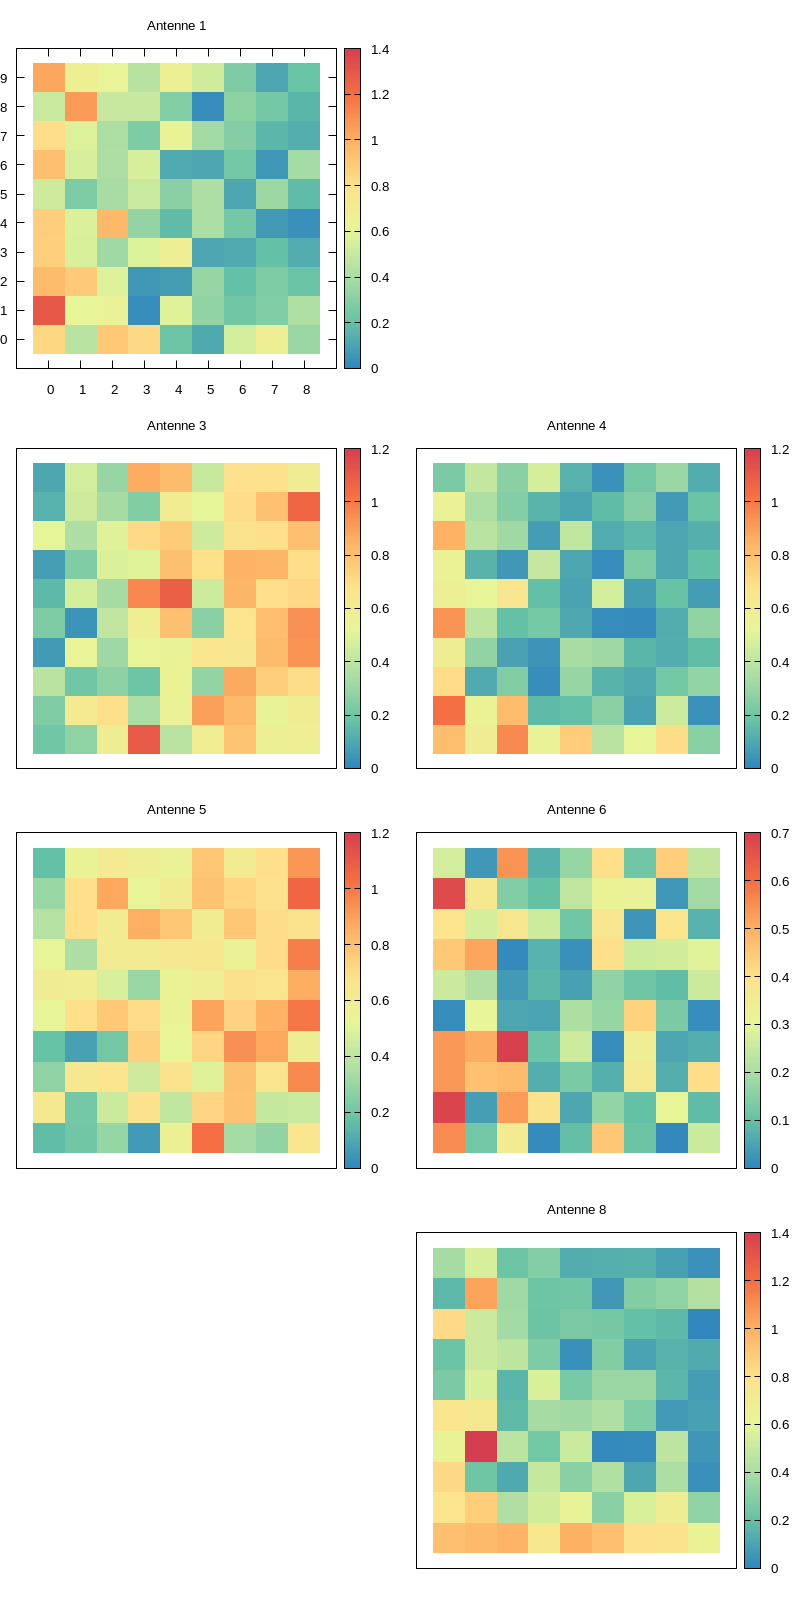
\includegraphics[width=0.65\textwidth]{img/resultRealData.png}
\end{figure}
%
Die Ergebnisse (Abbildung~\ref{fig:results2}) für reale Messwerte zeigen ein ähnliches Bild wie die idealen Messwerte. Eine steigende Gruppen- und Populationsgröße verbessert das Ergebnis in der Regel. Es fehlen die Plots der Antenne $2$ und $6$. Das liegt daran, dass diese beiden Antennen keine Messdaten lieferten. Es wurde der selbe Punkt ausgewählt, wie bei Vorstellung der ideal Messergebnisse. Damit sind die Ergebnisse unmittelbar vergleichbar. Genau wie bei den idealen Messdaten wurde der Ursprung der Kalibrierung als Messpunkt genommen. Das Ergebnis der realen Messwerte mutet sogar sicherer an, als das der idealen Phasenwerte. Der Grund dafür kann nicht exakt angegeben werden. Man kann sich dazu überlegen, da jeder Messwert ein Messrauschen enthält. Dieses Rauschen wird Teil des Modell und variiert dadurch unmittelbar die Fitnesslandschaft. Das Aussehen der Fitnesslandschaft wurde in Kapitel~\ref{sec:Komplexity2} untersucht. Weitere Untersuchungen und größere Messreihen müssen dieses Verhalten bestätigen.\\

Auch die neu kolorierte Darstellung der Ergebnisse in Abbildung~\ref{fig:results5} zeigt, wie die der idealen Messwerte, eine Verbesserung der Positionsbestimmung für steigende Populations- und Gruppengrößen.
%
%-----------------------------------------------------------------------------
%
\subsection{Evolutionsverlauf - real vs ideal}
%
Abschließend ist in Abbildung~\ref{fig:results3} der Verlauf der letzten beiden Experimente $2099$ und $3099$ gezeigt. Dort werden in $3$ Plots die Lösungen charakterisiert und die statistischen Eigenschaften sowie der Verlauf der Optimierung quantifiziert. Zu erkennen ist, dass sie die beiden Ergebnisse grundsätzlich ähneln. Unterschiede zeigen sich nur in Einzelheiten. So zeigt sich z.B., dass die Streuung der Parameter bei idealen Messwerten geringer ist, jedoch mehr Evaluationen notwendig waren. Allgemein zeigt sich der erwartete Verlauf einer evolutionären Optimierung.
%
%-----------------------------------------------------------------------------
%
\subsection{Performance}
%
Abschließend soll die Performance der Experimente gezeigt werden. Dabei wird die gleiche farbkodierte Darstellung verwendet, die auch bei den anderen Ergebnissen verwendet wird. Die Ausführungszeiten der Experimente sind in der Abbildung~\ref{fig:results6} und Abbildung~\ref{fig:results7} als Falschfarbenbild dargestellt. Die maximale Ausführungszeit betrug $\sim1200$~ms. Durch eine vernünftige Wahl von Populations- und Gruppengröße würde ein Ergebnis zwischen $400-600$~ms in Anspruch nehmen. Die Performance lässt sich durch Multithreading weiter verbessern.
%

%\textsc{First Letter}
%
%or
%
%{\scshape First Letter}

\begin{figure}[!ht]
	\centering
	\caption[Limitierte Ergebnisse - Ideale Messwerte]{ Alternative Visualisierung der zuvor gezeigten Ergebnisse, \textit{idealer} Messdaten. Zur besseren Übersicht wurde die Farbskala auf eine Wellenlänge reduziert. Abweichungen $\ge35$~cm werden rot eingefärbt. Gut $50\%$ der Werte führen nicht zu einen zufriedenstellenden Ergebnis. }
	\label{fig:results4}
	\vspace{3mm}
	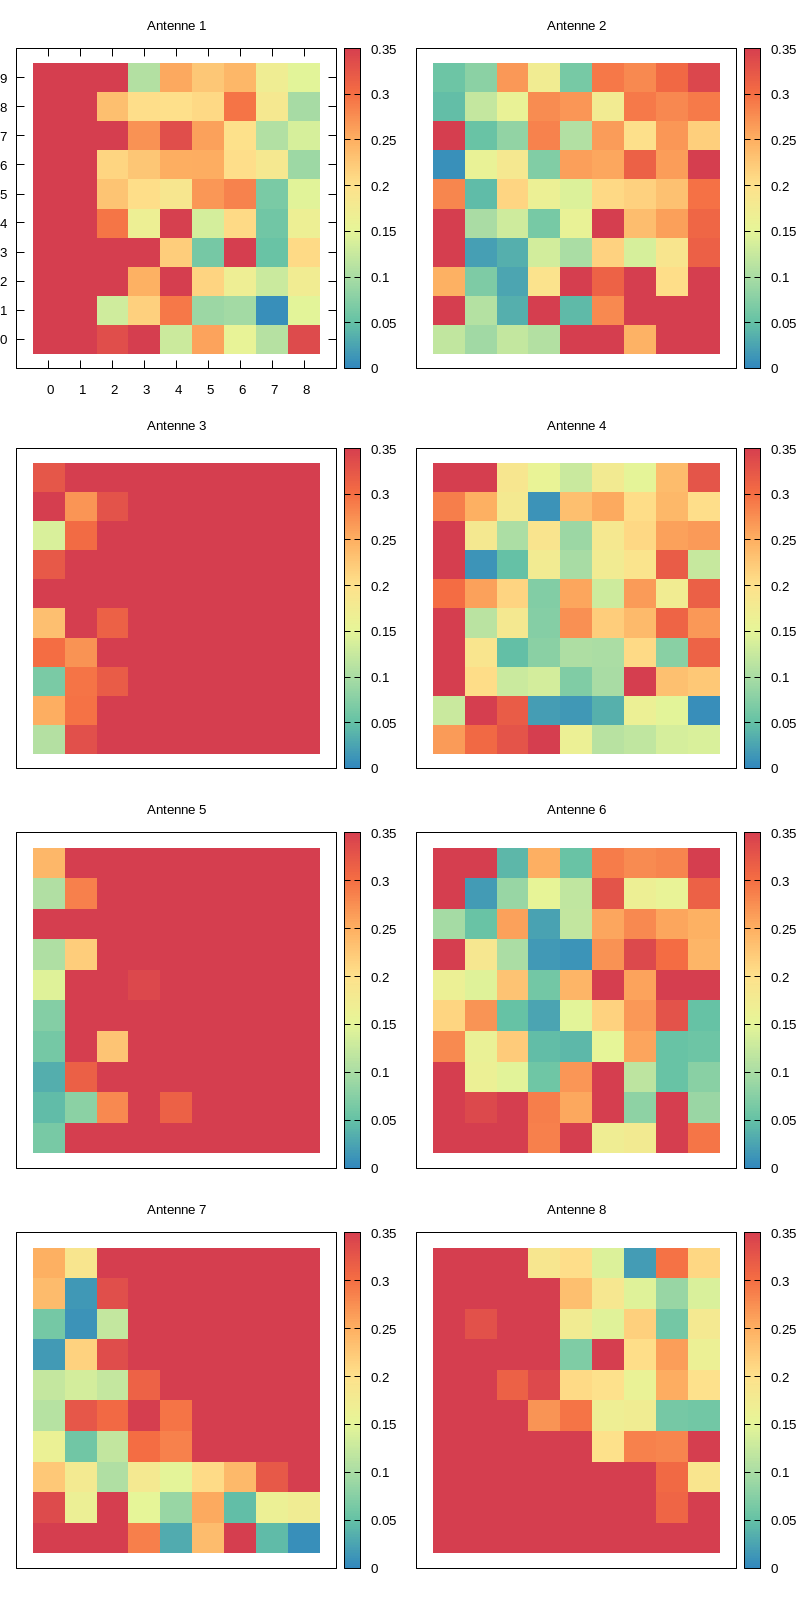
\includegraphics[width=0.65\textwidth]{img/limitedIdeal.png}
	

\end{figure}
%
\begin{figure}[!ht]
	\centering
	\caption[Limitierte Ergebnisse - Reale Messwerte]{Alternative Visualisierung der zuvor gezeigten Ergebnisse, \textit{realer} Messdaten.  Abweichungen $\ge35$~cm werden rot eingefärbt. Gut $50\%$ der Werte führen nicht zu einen zufriedenstellenden Ergebnis. Das Ergebnis gleicht dem der idealen Messdaten. }
	\label{fig:results5}
	\vspace{3mm}
	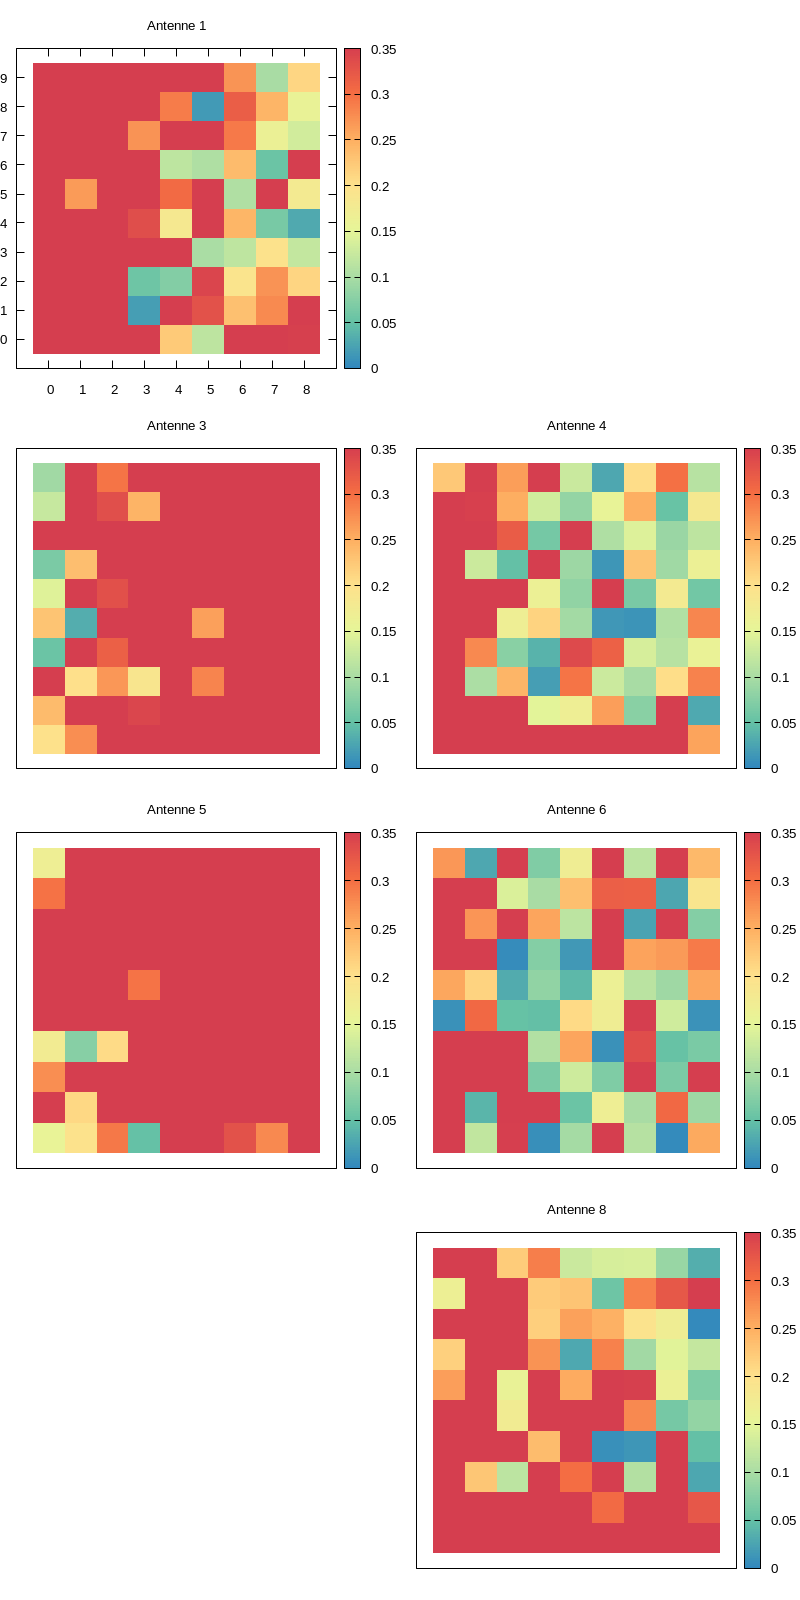
\includegraphics[width=0.65\textwidth]{img/limitedReal.png}
\end{figure}
%
\begin{landscape}
\begin{figure}[!ht]
	\caption[Evolutionsverlauf der Ergebnisse]{ Diese Grafik zeigt den Verlauf der Evolution. Es werden die Beiden letzten Experimente $2099$ (opben, ideale Messdaten) und $3099$ (unten, reale Messdaten) gezeigt. Diese Plots dienen nur der Einschätzung über den generellen Verlauf der Evolution. Es ist nicht sinnvoll sie für alle Experimente hier darzustellen. Anhand des Boxplots (Mitte) erkennend man, dass die Resultate für ideale Messwerte nicht so stark streuen, die Lösung der realen Messdaten ist den der idealen mind. Ebenbürtig. Es zeigt sich sogar, dass weniger Evaluationen der Zielfunktion bei den realen Werten nötig waren.}
	\label{fig:results3}
	\vspace{3mm}
	\centering
	\begin{subfigure}[t]{0.45\textheight}
	     \centering
	     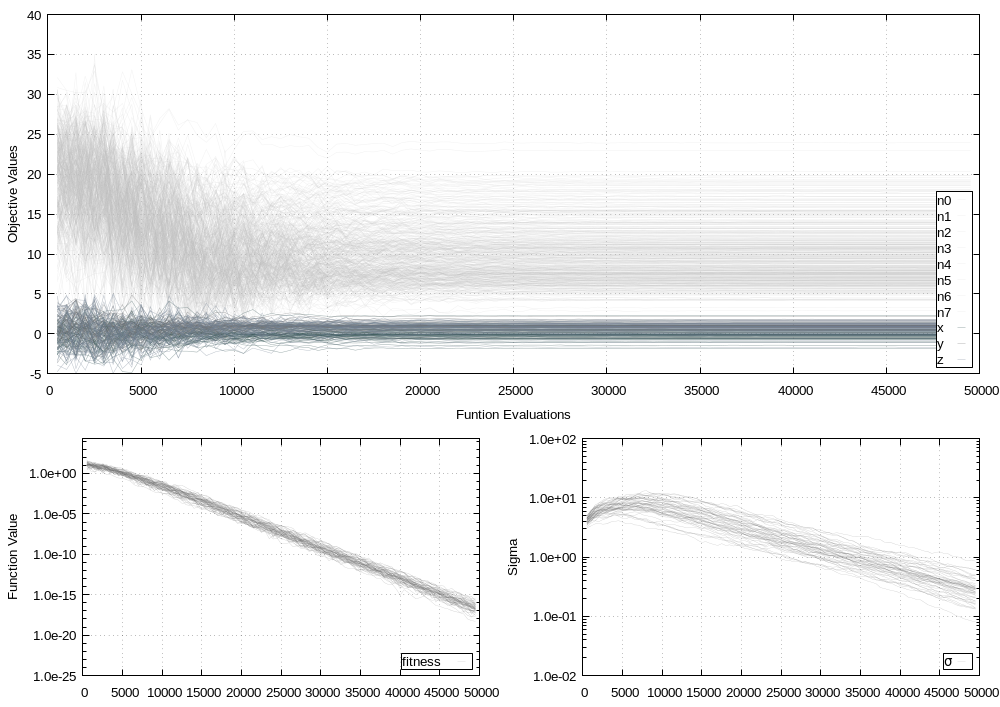
\includegraphics[width=\textwidth]{img/evo/lines2089.png}
	             \caption{Linienplot zur Analyse der Variablen und Optimierungsverlaufs.}
	%             \label{fig:abortedFinal_Calibration_Ant0_ES-boxes}
	\end{subfigure}
	\qquad
	\begin{subfigure}[t]{0.45\textheight}
		\centering
	     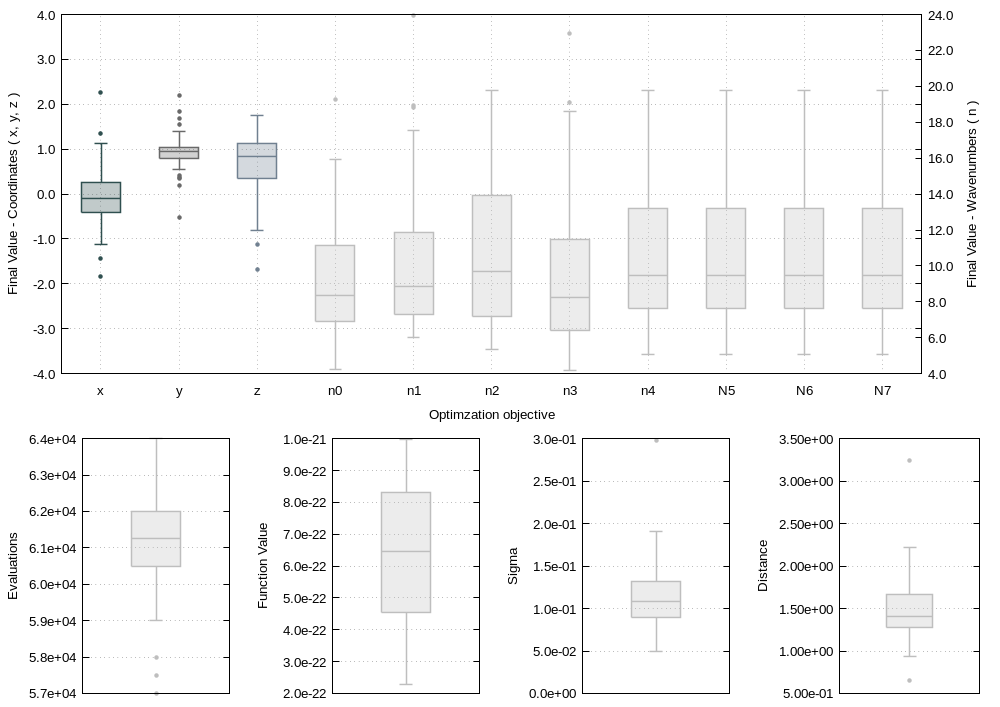
\includegraphics[width=\textwidth]{img/evo/boxes2089.png}
	     	    \caption{Boxplot zur Veranschaulichung der Lösungsstatistik }
	%			\label{fig:abortedFinal_Calibration_Ant0_ES-boxes}
	\end{subfigure}
	\qquad
	\begin{subfigure}[t]{0.45\textheight}
			\centering
	   \includegraphics[width=\textwidth]{img/evo/Scatter2089.png}
	   	       \caption{Streuplot zur Untersuchung von Abhängigkeiten der Parameter}
	%			\label{fig:abortedFinal_Calibration_Ant0_ES-boxes}
	\end{subfigure}
	\vspace{5mm}
\\
	\centering
	\begin{subfigure}[t]{0.45\textheight}
	     \centering
	     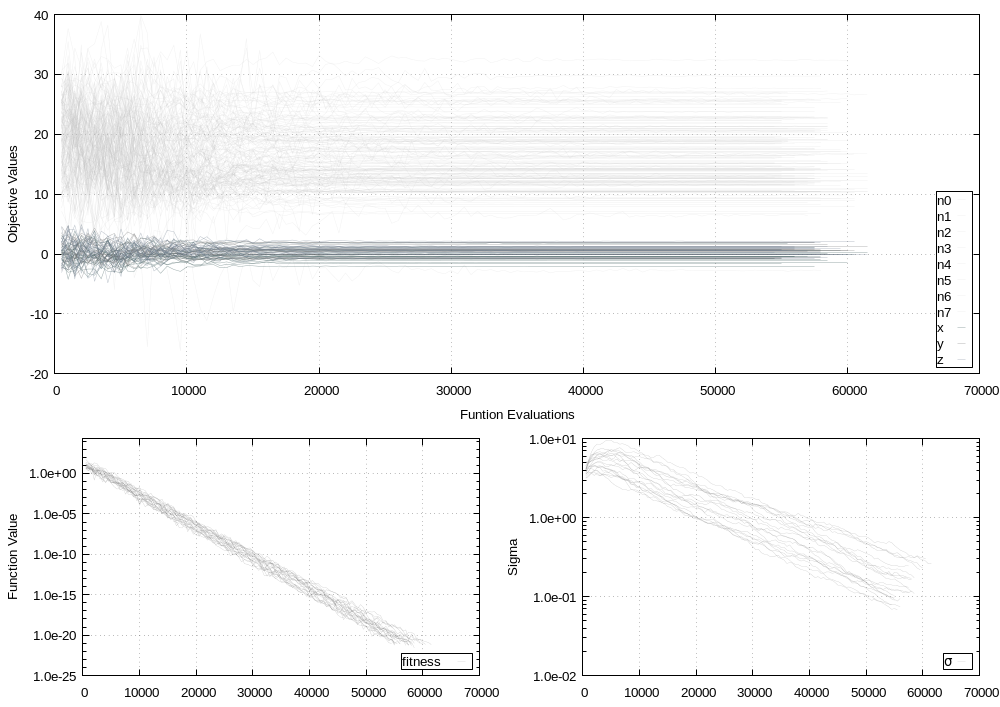
\includegraphics[width=\textwidth]{img/evo/lines4089.png}
	             \caption{Linienplot zur Analyse der Variablen und Optimierungsverlaufs.}
	%             \label{fig:abortedFinal_Calibration_Ant0_ES-boxes}
	\end{subfigure}
	\qquad
	\begin{subfigure}[t]{0.45\textheight}
		\centering
	     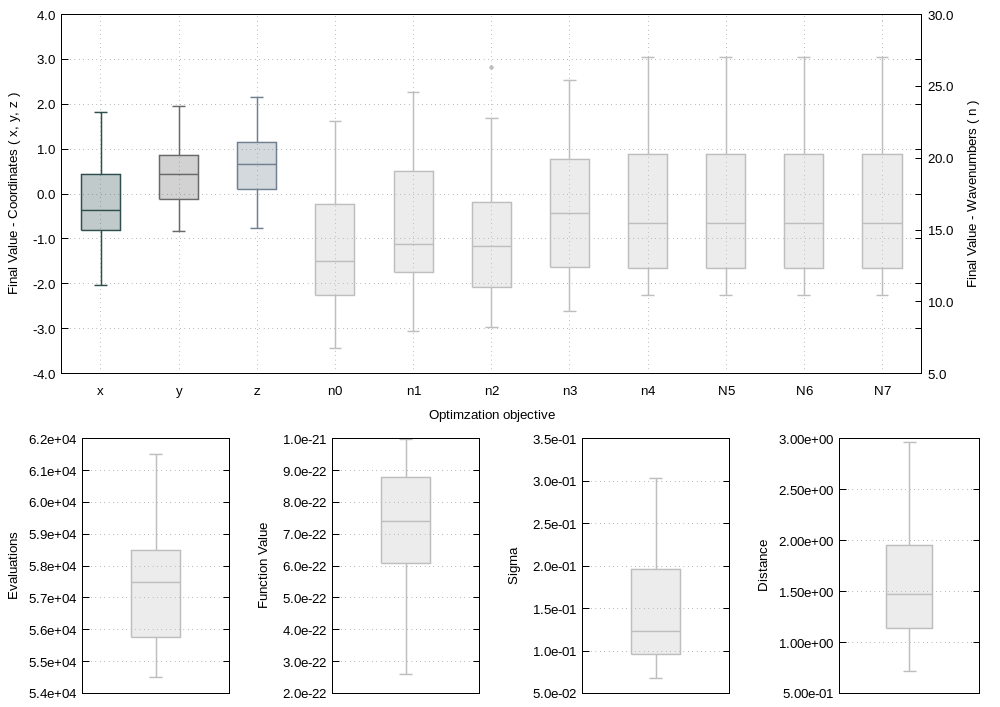
\includegraphics[width=\textwidth]{img/evo/boxes4089.png}
	     	    \caption{Boxplot zur Veranschaulichung der Lösungsstatistik }
	%			\label{fig:abortedFinal_Calibration_Ant0_ES-boxes}
	\end{subfigure}
	\qquad
	\begin{subfigure}[t]{0.45\textheight}
			\centering
	   \includegraphics[width=\textwidth]{img/evo/Scatter4089.png}
	   	       \caption{Streuplot zur Untersuchung von Abhängigkeiten der Parameter}
	%			\label{fig:abortedFinal_Calibration_Ant0_ES-boxes}
	\end{subfigure}

\end{figure}
\newpage
\end{landscape}
%
\begin{figure}[!ht]
	\centering
	\caption[Performance Ergebnisse - Ideale Messwerte]{ Visualisierung der Performance. Die Resultate wurde in einer virtuellen Umgebung generiert. Aufgrund limitierter Ressourcen (nur ein Prozessor verfügbar). Konnte die Multithreading-Fähigkeit nicht genutzt werden. Die Ausführungszeiten für vernünftige Konfigurationen liegen bei $\sim800$~ms ohne Threading. Gut zu erkennen ist, dass mit steigendem Aufwand die Ausführungszeit, wie erwartet steigt. }
	\label{fig:results6}
	\vspace{3mm}
	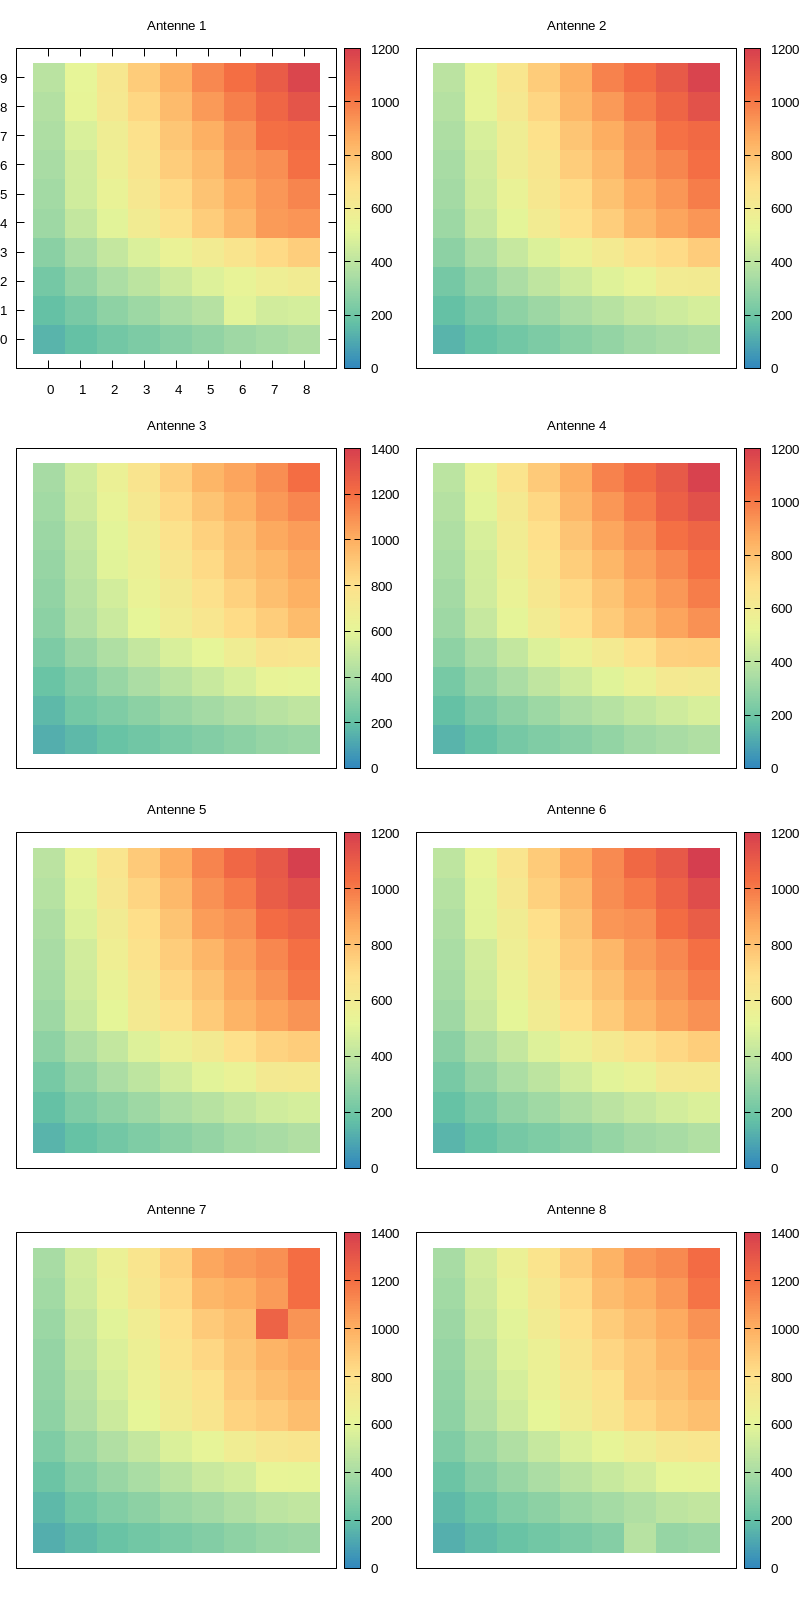
\includegraphics[width=0.65\textwidth]{img/resultstiming.png}
\end{figure}
%
%
\begin{figure}[!ht]
	\centering
	\caption[Performance Ergebnisse -- Reale Messwerte]{ Keine Überraschungen hier. Mit zunehmender Komplexität zeigt sich eine Zunahme der Ausführungszeit. Gleiches Ergebnis wie bei den idealen Messdaten. }
	\label{fig:results7}
	\vspace{3mm}
	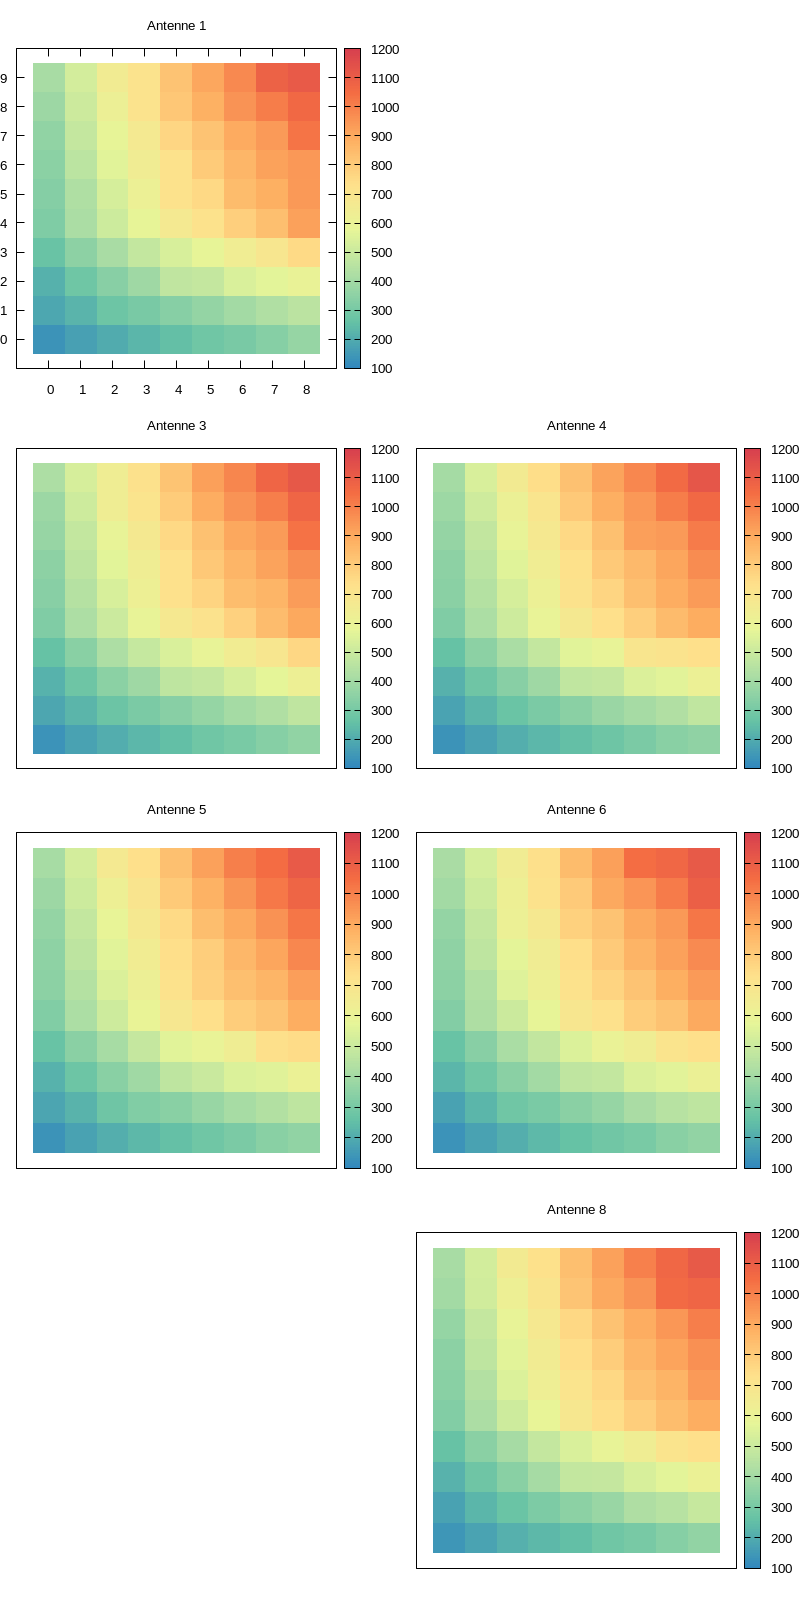
\includegraphics[width=0.65\textwidth]{img/resultstimingreal.png}
\end{figure}
%